\documentclass[11pt,compress,t,notes=noshow, xcolor=table]{beamer}
\usepackage[]{graphicx}\usepackage[]{color}
% maxwidth is the original width if it is less than linewidth
% otherwise use linewidth (to make sure the graphics do not exceed the margin)
\makeatletter
\def\maxwidth{ %
  \ifdim\Gin@nat@width>\linewidth
    \linewidth
  \else
    \Gin@nat@width
  \fi
}
\makeatother

\definecolor{fgcolor}{rgb}{0.345, 0.345, 0.345}
\newcommand{\hlnum}[1]{\textcolor[rgb]{0.686,0.059,0.569}{#1}}%
\newcommand{\hlstr}[1]{\textcolor[rgb]{0.192,0.494,0.8}{#1}}%
\newcommand{\hlcom}[1]{\textcolor[rgb]{0.678,0.584,0.686}{\textit{#1}}}%
\newcommand{\hlopt}[1]{\textcolor[rgb]{0,0,0}{#1}}%
\newcommand{\hlstd}[1]{\textcolor[rgb]{0.345,0.345,0.345}{#1}}%
\newcommand{\hlkwa}[1]{\textcolor[rgb]{0.161,0.373,0.58}{\textbf{#1}}}%
\newcommand{\hlkwb}[1]{\textcolor[rgb]{0.69,0.353,0.396}{#1}}%
\newcommand{\hlkwc}[1]{\textcolor[rgb]{0.333,0.667,0.333}{#1}}%
\newcommand{\hlkwd}[1]{\textcolor[rgb]{0.737,0.353,0.396}{\textbf{#1}}}%
\let\hlipl\hlkwb

\usepackage{framed}
\makeatletter
\newenvironment{kframe}{%
 \def\at@end@of@kframe{}%
 \ifinner\ifhmode%
  \def\at@end@of@kframe{\end{minipage}}%
  \begin{minipage}{\columnwidth}%
 \fi\fi%
 \def\FrameCommand##1{\hskip\@totalleftmargin \hskip-\fboxsep
 \colorbox{shadecolor}{##1}\hskip-\fboxsep
     % There is no \\@totalrightmargin, so:
     \hskip-\linewidth \hskip-\@totalleftmargin \hskip\columnwidth}%
 \MakeFramed {\advance\hsize-\width
   \@totalleftmargin\z@ \linewidth\hsize
   \@setminipage}}%
 {\par\unskip\endMakeFramed%
 \at@end@of@kframe}
\makeatother

\definecolor{shadecolor}{rgb}{.97, .97, .97}
\definecolor{messagecolor}{rgb}{0, 0, 0}
\definecolor{warningcolor}{rgb}{1, 0, 1}
\definecolor{errorcolor}{rgb}{1, 0, 0}
\newenvironment{knitrout}{}{} % an empty environment to be redefined in TeX

\usepackage{alltt}
\newcommand{\SweaveOpts}[1]{}  % do not interfere with LaTeX
\newcommand{\SweaveInput}[1]{} % because they are not real TeX commands
\newcommand{\Sexpr}[1]{}       % will only be parsed by R
\newcommand{\xmark}{\ding{55}}%


\usepackage[english]{babel}
\usepackage[utf8]{inputenc}

\usepackage{dsfont}
\usepackage{verbatim}
\usepackage{amsmath}
\usepackage{amsfonts}
\usepackage{amssymb}
\usepackage{bm}
\usepackage{csquotes}
\usepackage{multirow}
\usepackage{longtable}
\usepackage{booktabs}
\usepackage{enumerate}
\usepackage[absolute,overlay]{textpos}
\usepackage{psfrag}
\usepackage{algorithm}
\usepackage{algpseudocode}
\usepackage{eqnarray}
\usepackage{arydshln}
\usepackage{tabularx}
\usepackage{placeins}
\usepackage{tikz}
\usepackage{setspace}
\usepackage{colortbl}
\usepackage{mathtools}
\usepackage{wrapfig}
\usepackage{bm}
\usepackage{amsmath}
\usepackage{pifont}
\usepackage[round]{natbib}
\usepackage{hyperref}

\usetikzlibrary{shapes,arrows,automata,positioning,calc,chains,trees, shadows}
\tikzset{
  %Define standard arrow tip
  >=stealth',
  %Define style for boxes
  punkt/.style={
    rectangle,
    rounded corners,
    draw=black, very thick,
    text width=6.5em,
    minimum height=2em,
    text centered},
  % Define arrow style
  pil/.style={
    ->,
    thick,
    shorten <=2pt,
    shorten >=2pt,}
}

\usepackage{subfig}

% Defines macros and environments
\usepackage{../../style/lmu-lecture}


\let\code=\texttt
\let\proglang=\textsf

\setkeys{Gin}{width=0.9\textwidth}

\setbeamertemplate{frametitle}{\expandafter\uppercase\expandafter\insertframetitle}

% basic latex stuff
\newcommand{\pkg}[1]{{\fontseries{b}\selectfont #1}} % fontstyle for R packages

% Often used in exercise Rnw files, still relevant?
\newcommand{\lz}{\vspace{0.5cm}} % vertical space
\newcommand{\dlz}{\vspace{1cm}}  % double vertical space

% Unused and about to be deleted
\newcommand{\oneliner}[1] % Oneliner for important statements
{\begin{block}{}\begin{center}\begin{Large}#1\end{Large}\end{center}\end{block}}


%--------------------%
%  New environments  %
%--------------------%

 % Frame with breaks and verbatim // this is used very often
\newenvironment{vbframe}
{
\begin{frame}[containsverbatim,allowframebreaks]
}
{
\end{frame}
}

% Frame with verbatim without breaks (to avoid numbering one slided frames)
% This is not used anywhere but I can see it being useful
\newenvironment{vframe}
{
\begin{frame}[containsverbatim]
}
{
\end{frame}
}

% Itemize block
\newenvironment{blocki}[1]
{
\begin{block}{#1}\begin{itemize}
}
{
\end{itemize}\end{block}
}

%--------------%
%  Citebutton  %
%--------------%
% Example usage (from slides-cart-discussion.tex)
% \citebutton{Breiman, 1984}{https://www.taylorfrancis.com/books/mono/10.1201/9781315139470/classification-regression-trees-leo-breiman}
\newcommand{\citebutton}[2]{%
\NoCaseChange{\resizebox{!}{9pt}{\protect\beamergotobutton{\href{#2}{#1}}}}%
}

% textcolor that works in mathmode
% https://tex.stackexchange.com/a/261480
% Used e.g. in forests/slides-forests-bagging.tex
% [...] \textcolor{blue}{\tfrac{1}{M}\sum^M_{m} [...]
\makeatletter
\renewcommand*{\@textcolor}[3]{%
  \protect\leavevmode
  \begingroup
    \color#1{#2}#3%
  \endgroup
}
\makeatother






\newcommand{\titlefigure}{figure_man/mckenzie_ai.jpeg}
\newcommand{\titlecaption}{\tiny Image via \url{www.vpnsrus.com}}
\newcommand{\learninggoals}{
\item Understand basic terminology of and connections between ML, AI, DL and statistics
\item Know the main directions of ML: Supervised, Unsupervised and Reinforcement Learning}


\title{Introduction to Machine Learning}
% \author{Bernd Bischl, Christoph Molnar, Daniel Schalk, Fabian Scheipl}
\institute{\href{https://compstat-lmu.github.io/lecture_i2ml/}{compstat-lmu.github.io/lecture\_i2ml}}
\date{}

\begin{document}

\lecturechapter{ML-Basics: What is Machine Learning?}
\lecture{Introduction to Machine Learning}

\sloppy

% ------------------------------------------------------------------------------

\begin{frame}{Machine Learning is changing our world}

\begin{itemize}

  \item Search engines learn what you want
  
  \item Recommender systems learn your taste in books, music, movies,...
  
  \item Algorithms do automatic stock trading
  
  \item Google Translate learns how to translate text
  
  \item Siri learns to understand speech
  
  \item DeepMind beats humans at Go
  
  \item Cars drive themselves
  
  % \item Medicines are developed faster
  
  \item Smart-watches monitor your health
  
  \item Election campaigns use algorithmically targeted ads to influence voters
  
  \item Data-driven discoveries are made in physics, biology, genetics, 
  astronomy, chemistry, neurology,...
  
  \item ...
  
\end{itemize}

\end{frame}

% ------------------------------------------------------------------------------

\begin{frame}{The World of Artificial Intelligence}

... and the connections to Machine Learning and Deep Learning

% Machine learning is a branch of statistics and computer science. 

\begin{center}

  \begin{figure}
    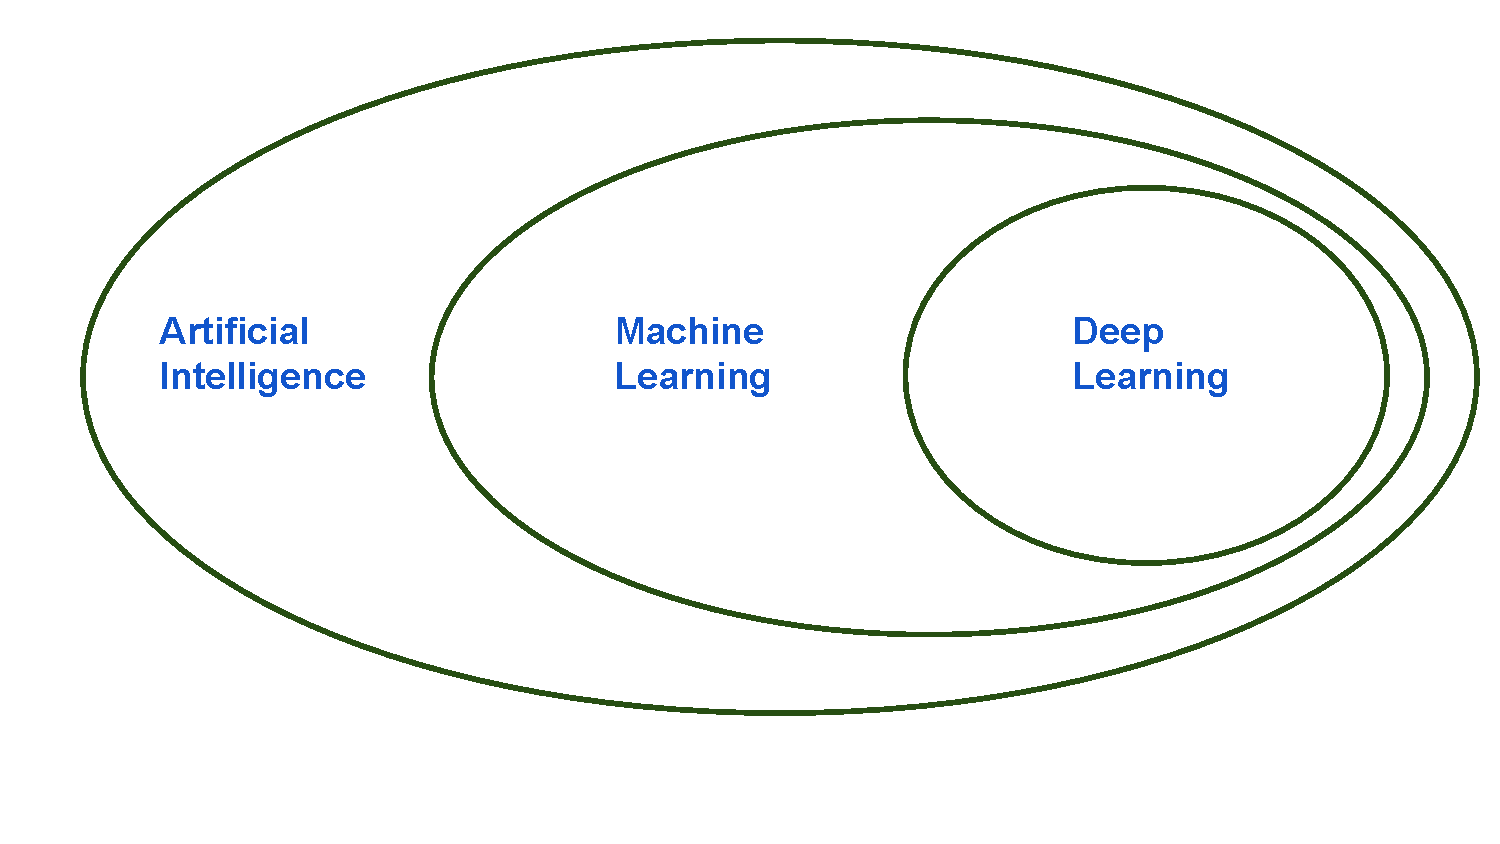
\includegraphics[width=0.7\textwidth]{figure_man/learning} 
  \end{figure}

  \lz

Many people are confused what these terms actually mean. 

\lz

And what does all this have to do with statistics?

  % Machine Learning is a method of teaching computers to make predictions based 
  % on some data.

%  A computer program is said to \textbf{learn} from experience E with respect to
%  some task T and some performance measure P, if its performance on T, as 
%  measured by P, improves with experience E. \\
%  
%  \begin{footnotesize}
%  \emph{Tom Mitchell, Carnegie Mellon University, 1998}
%  \end{footnotesize}
  
  \end{center}
  
\end{frame}

% ------------------------------------------------------------------------------

\begin{frame}{Artificial Intelligence}

\begin{itemize}
	\item AI is a general term for a very large and rapidly developing field.
	\item There is no strict definition of AI, but it's often used when machines are trained to perform on tasks which until that time could only be solved by humans or are very difficult and assumed to require "intelligence".
    \item AI started in the 1940s - when the computer was invented. Scientists like 
        Turing and John von Neumann immediately asked the question:
        If we can formalize computation, can we use computation to formalize "thinking"?
	\item AI includes machine learning, natural language processing, computer vision, robotics, planning, search, game playing, intelligent agents, and much more.
    \item Nowadays, AI is a "hype" term that many people use when they should probably say: ML or ... basic data analysis.
\end{itemize}
  
\end{frame}

% ------------------------------------------------------------------------------

\begin{frame}{Machine Learning}

\begin{columns}
\begin{column}{0.65\textwidth}
\begin{center}
  % FIGURE SOURCE: https://www.oreilly.com/library/view/java-deep-learning/9781788997454/assets/899ceaf3-c710-4675-ae99-33c76cd6ac2f.png
  % \includegraphics[width=0.7\textwidth]{figure_man/l}
  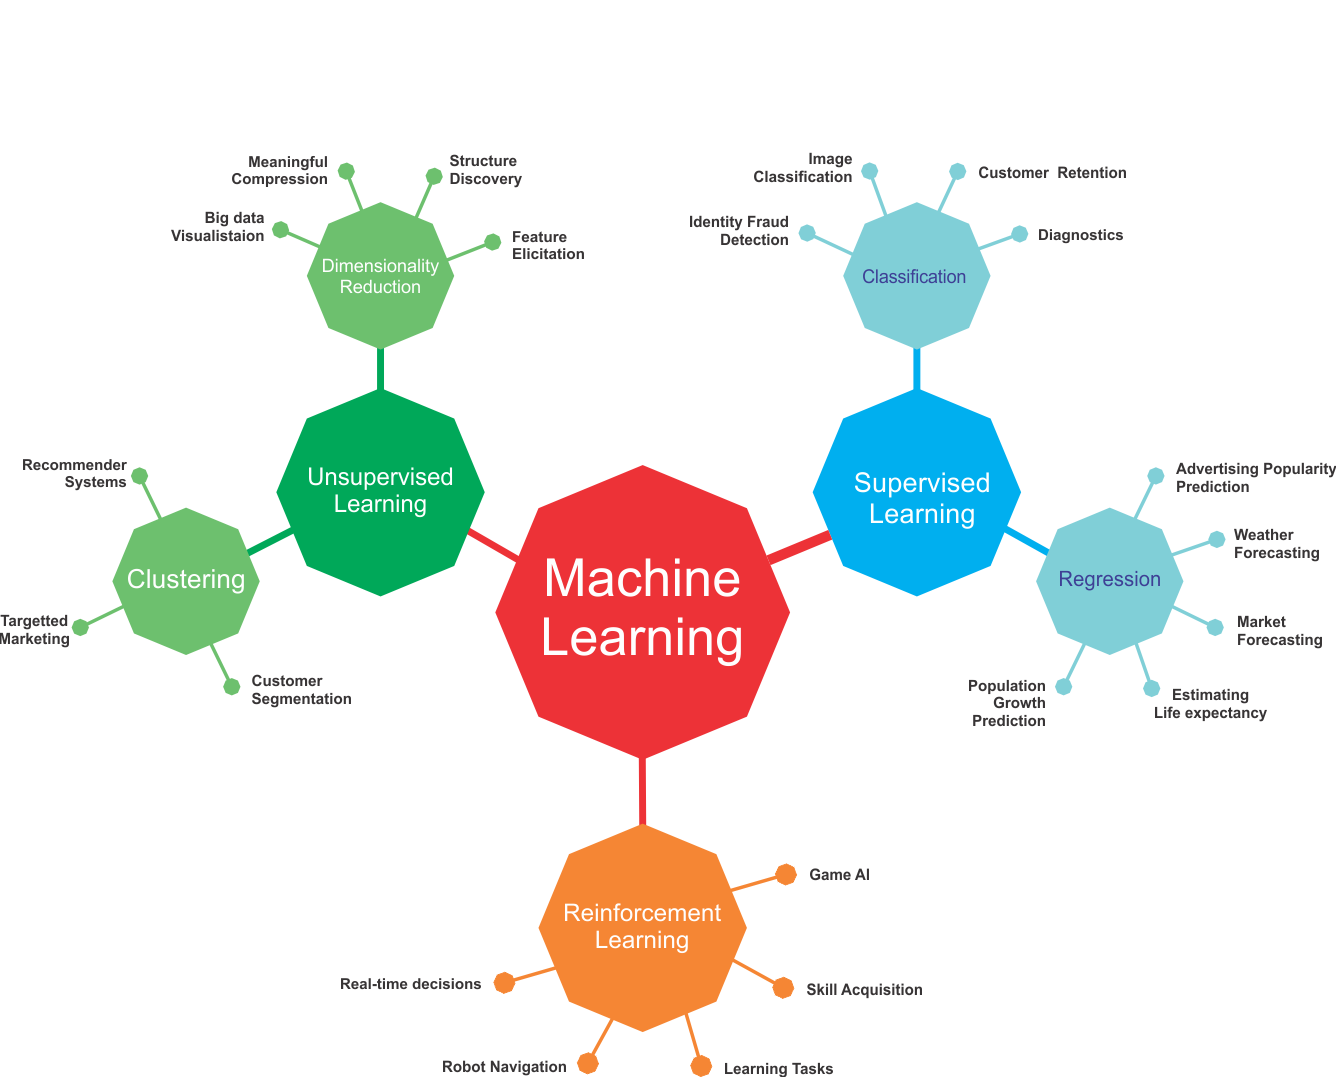
\includegraphics[trim=0 0 0 0,clip,width=\textwidth]{figure_man/whatisml.png}\\[3ex]
  \tiny{Image via \url{https://www.oreilly.com/library/view/java-deep-learning/9781788997454/assets/899ceaf3-c710-4675-ae99-33c76cd6ac2f.png}}
\end{center}
\end{column}
\begin{column}{0.45\textwidth}
\begin{footnotesize}
\begin{itemize}
    % \item Mainly includes supervised, unsup. and reinforcement learning.
	\item Mathematically well-defined and solves reasonably narrow tasks.
	\item ML algorithms usually construct predictive/decision models from data, instead of explicitly programming them.
    \item A computer program is said to learn from experience E with respect to
  some task T and some performance measure P, if its performance on T, as 
  measured by P, improves with experience E. \\
  \begin{footnotesize}
  \emph{Tom Mitchell, Carnegie Mellon University, 1998}
  \end{footnotesize}
\end{itemize}
\end{footnotesize}
\end{column}
\end{columns}
  
\end{frame}

\begin{vbframe}{Deep Learning}

\begin{itemize}
\item DL is a subfield of ML which studies neural networks.
\item Artificial neural networks (ANNs) might have been (roughly) inspired by the human brain, but they are simply a certain model class of ML.
\item ANNs have been studied for decades. DL uses more layers, 
        specific neurons were invented for images and tensors and many computational 
        improvements allow training on large data.
	% \item The term refers to the fact that rather complex neural networks, i.e. \emph{deep} networks are used
\item DL can be used on tabular data, but typical applications are images, texts or signals. 
\item The last 10-15 years have produced remarkable results and imitations of human ability, where the result looked intelligent. 
\end{itemize}

\lz

"Any sufficiently advanced technology is indistinguishable from magic."
\begin{footnotesize}
\emph{Arthur C. Clarke's 3rd law}
\end{footnotesize}
 

\end{vbframe}

% ------------------------------------------------------------------------------

\begin{frame}{ML vs. Stats}


\begin{itemize}
	\item ML and Statistics have historically been developed in different fields, but many
      methods and especially the mathematical foundations are equivalent.
	\item Traditionally, models from ML focused more on precise predictions whereas models from statistics focused more on the ability to interpret the patterns that generated the data and the ability to derive sound inference.
	\item Nowadays, ML and predictive modelling in statistics basically work on the same problems with the same tools.
    \item Unfortunately, the communities are still divided, don't talk to each other as much as they should and everyone is confused due to different terminology for the same concepts.
        % from both worlds can be used for similar tasks because ML models have gained in interpretability and statistics models have gained in predictive power
    \item Most parts of ML we could also call:\\Nonparametric statistics plus efficient numerical optimization.
\end{itemize}

\end{frame}


\begin{vbframe}{Unsupervised learning}
\begin{itemize}
  \item Data without labels $y$
  \item Search for patterns within the inputs $x$
  \item \textit{Unsupervised} as there is no \enquote{true} output
      we can optimize against
\end{itemize}

\lz

\begin{columns}
\begin{column}{0.45\textwidth}
\begin{center}
    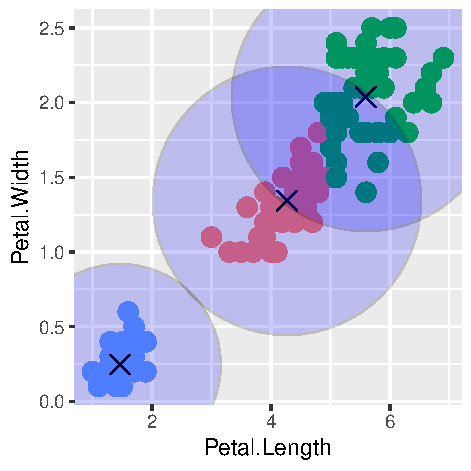
\includegraphics[width=\textwidth]{figure/unsup.pdf}
\end{center}
\end{column}
\begin{column}{0.55\textwidth}
% \begin{footnotesize}
\begin{itemize}
    \item Dimensionality reduction (PCA, Autoencoders ...);\\ 
        compress information in $\mathcal X$
    \item Clustering: group similar observations
    \item Outlier detection, anomaly detection
    \item Association rules
\end{itemize}
% \end{footnotesize}
\end{column}
\end{columns}
\end{vbframe}

\begin{vbframe}{Reinforcement learning}

RL is a general-purpose framework for AI.
At each time step an \emph{agent} interacts with \emph{environment}. 
It: observes state; receives reward; executes action.
  % \end{itemize}

\begin{center}
  %image from rcourses
  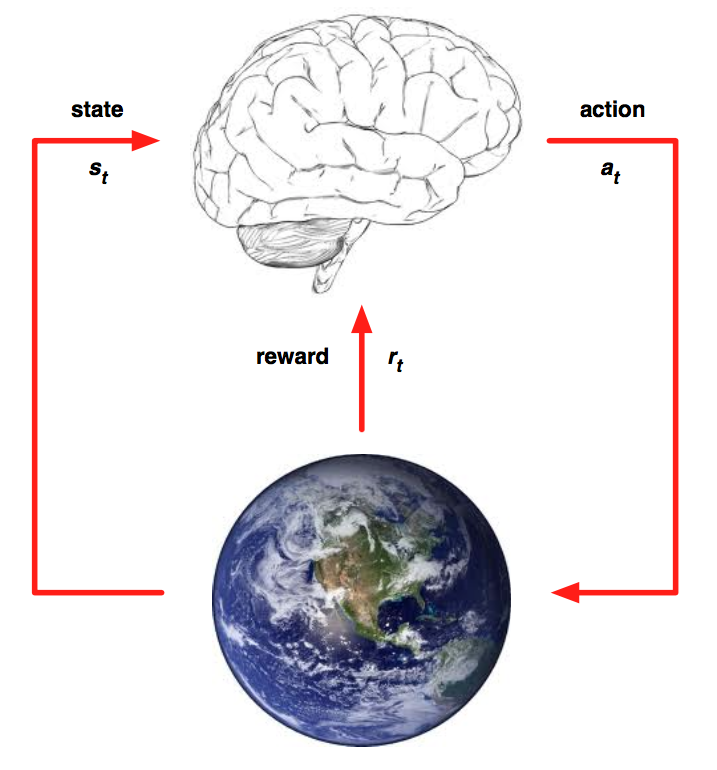
\includegraphics[height=0.4\textheight,keepaspectratio]{figure_man/state_action_reward_diagram.png}
\end{center}


\begin{itemize}
\item Goal: Select actions to maximize future reward.
 % \item Inputs are observations and feedback (rewards or punishments) from
  % interacting with an environment
\item Reward signals may be sparse, noisy and delayed.
\end{itemize}

% Example: train neural net to play mario kart (environment)
\end{vbframe}


% ------------------------------------------------------------------------------


% ------------------------------------------------------------------------------

\begin{frame}{What comes next}

\begin{itemize}

\item We will deal with \textbf{supervised learning} for regression 
and classification: predicting labels $y$ based on features $x$, using 
patterns that we learned from labeled data.
  
  \item First, we will go through fundamental concepts in supervised ML: 
  \begin{itemize}
  
    \item What kind of "data" do we learn from?
    \item How can we formalize the goal of learning?
    \item What is a "prediction model"?
    \item How can we quantify "predictive performance"?
    \item What is a "learning algorithm" 
    \item How can we operationalize learning?
  
  \end{itemize}
  
  \item We will also look at a couple of fairly simple ML models to obtain a
  basic understanding.
  
  \item More complex stuff comes later.
  
\end{itemize}

\end{frame}


% ------------------------------------------------------------------------------

\endlecture
\end{document}
